\documentclass[a4paper,12pt,russian]{article}
\usepackage[T2A]{fontenc}
\usepackage[utf8]{inputenc}
\usepackage[russian]{babel}
\usepackage[a4paper,left=2cm, right=2cm, top=2cm, bottom=2cm]{geometry}
\usepackage{graphicx}
\graphicspath{{figures/}}
\DeclareGraphicsExtensions{.pdf,.png,.jpg}
\usepackage{amsfonts}
\usepackage{amsmath}
\usepackage{multirow}
\usepackage{multicol}
\usepackage{caption} 

\linespread{1.3}

% дополнительно
\usepackage{algorithm}
\usepackage{algpseudocode}
\usepackage{multirow}
\usepackage{listings}
\usepackage{xcolor}
\usepackage{wasysym}


\begin{document}

\begin{center}
	\textbf{A GLOBAL OPTIMIZATION ALGORITHM FOR \break
    TUNING HYPERPARAMETERS OF MACHINE LEARNING METHODS} 
\end{center}

\begin{center}
{M.A.~Usova, I.G.~Lebedev, A.A.~Shtanyuk, K.A.~Barkalov}
\end{center}

\begin{center}
{Lobachevsky State University, 603022, Nizhny Novgorod, Russia}
\end{center}
\begin{small}

% аннотация англ.
\colorbox{orange}{исправить в соответсвии с введением и экспериментами ->}
The paper discusses the problem of finding a global minimum of a function that may be multiextremal, non-differentiable, given in the form of a ``black box'' and computable only in some part of the search domain. In this case, each computation of the objective function value at some point of the feasible domain may require significant computing resources. The objective function is assumed to satisfy the Lipschitz condition.
The existence of subdomains where the objective function is undefined can be interpreted as the existence of some hidden, a priori unknown constraints of the problem. Such an effect can occur when solving applied problems due to the specific features of the optimized object or modeling method (for example, numerical instability of the method for some combination of parameters). In such subdomains, it is impossible to correctly perform numerical modeling and estimate the value of the objective function. A special case is the problem of tuning hyperparameters of artificial intelligence (AI) and machine learning (ML) methods. In these problems, the efficiency (in a given metric) of the resulting solution for different values of hyperparameters can be quite different. Moreover, the computational complexity of tuning makes the exhaustive search practically inapplicable. These features required the development of various methods for intelligent automatic tuning of hyperparameters. At the same time, the problem of existence of unacceptable combinations of hyperparameters, which was not particularly important in the case of manual tuning, has become a stumbling block for many frameworks using intelligent tuning methods.
Our goal is to develop an algorithm in which the absence of a value of the objective function at some point should not lead to its incorrect operation. The proposed approach to solving such problems extends the information-statistical global search algorithm (GSA). This algorithm solves multidimensional problems by reducing them to one-dimensional optimization problems using space-filling curves (Peano curves).
In this study, new rules for processing search intervals with no objective function values at their boundary points were proposed. The calculation of the characteristic of an interval with two non-computable points is based on the interval length. To minimize the number of redundant trials in subdomains where the function is not defined, we used a special method parameter $\alpha$ that regulates the number of trial points in these subdomains. The calculation of the characteristic of an interval with non-computable and computable points is performed according to the rules for working with a boundary interval. The article provides a detailed description of a modified global search algorithm for solving the class of problems under consideration.
The implementation of the global search algorithm for the case of a not-everywhere computable objective function (GSA-N) was based on the iOpt open source framework of intelligent optimization methods.
To carry out the experiments, a generator of test problems with hidden constraints GKLS-HC was developed. It is based on the GKLS generator, which allows generating multi-extremal functions with specified properties (number of minima, their regions of attraction, etc.). In the GKLS-HC generator, these functions were spoiled by areas of non-computability in the form of ellipsoids (the coordinates of centers and radii were generated randomly).
The experimental results presented in the paper, obtained on a series of GKLS-HC test problems, demonstrate the reliability of global search and the efficiency of the developed algorithm. By adjusting the parameter $\alpha$, it was possible to achieve the same speed of GSA-N operation as the basic GSA.
The paper also considered the behavior of global optimization algorithms of the \textit{scipy.optimize} library when solving problems with non-computable domains. In this study, the differential evolution and brute force methods showed the worst results, failing to solve this type of problem at all. The DIRECT and SHGO methods, although they solved the problems, were less effective than the developed GSA-N.
In addition, the paper presents the results of numerical experiments obtained when tuning the hyperparameters of the LinearSVC method used to solve the classification problem on the well-known Iris dataset.

%Here is the text of the extended annotation in English, ranging from 4000 to 8000 characters.
%В статье обсуждается проблема поиска глобального минимума функции, которая может быть многоэкстремальной, недифференцируемой, более того, заданной в форме «черного ящика» и вычислимой лишь в некоторой части области поиска. При этом каждое вычисление функции в некоторой точке допустимой области может требовать значительных вычислительных ресурсов. О целевой функции известно лишь что она удовлетворяет условию Липшица.
%Наличие подобластей, в которых целевая функция является неопределенной, можно интерпретировать как наличие некоторых скрытых, заранее неизвестных ограничений задачи. Такой эффект может возникать при решении прикладных задач в силу особенностей оптимизируемого объекта или метода моделирования (например, численная нестабильность метода при определенном сочетании параметров). В таких подобластях невозможно корректно провести численное моделирование и оценить значение целевой функции. Частным случаем является задача настройки гиперпараметров методов искусственного интеллекта (ИИ) и машинного обучения (МО). Во многих случаях разница в эффективности (в заданной метрике) получаемого решения при разных значениях гиперпараметров может быть достаточно значительной. При этом вычислительная сложность настройки делает невозможным использование полного перебора. Данные особенности определили необходимость разработки различных методов интеллектуального автоматического подбора гиперпараметров. При этом проблема возникновения недопустимых комбинаций гиперпараметров, которая не имела особого значения в случае «ручной» настройки, для многих фреймворков, использующих методы интеллектуальной настройки, стала камнем преткновения.
%Нашей целью является разработка алгоритма, в котором отсутствие значения целевой функции в некоторой точке не должно приводить к его некорректной работе. Предлагаемый подход к решению такого рода задач является расширением информационно-статистического алгоритма глобального поиска (АГП). Данный алгоритм предполагает решение многомерных задач посредством их сведения к задачам одномерной оптимизации при помощи кривых, заполняющих пространство (кривых Пеано). В рамках данного исследования были предложены новые правила обработки поисковых интервалов, в граничных точках которых отсутствуют значения целевой функции. Расчёт характеристики интервала с двумя невычислимыми точками производится, основываясь на длине интервала. Для минимизации количества избыточных испытаний в областях, в которых функция не определена, при таком подходе используется специальный параметр метода, позволяющий регулировать число точек испытаний в области невычислимости.  Расчёт характеристики интервала с невычислимой и вычислимой точками производится по правилам работы с граничным интервалом. В статье изложено подробное описание модифицированного алгоритма глобального поиска для решения исследуемого класса задач.
%Программная реализация алгоритма глобального поиска на случай не всюду вычислимой целевой функции (АГП-Н) была выполнена на базе фреймворка методов интеллектуальной эвристической оптимизации iOpt открытым исходным кодом.
%Для проведения экспериментов был разработан генератор задач со скрытыми ограничениями GKLSHiddenConstraint, взявший за основу генератор GKLS, позволяющий порождать задачи многоэкстремальной оптимизации с заранее известными свойствами. Данные функции были дополнены сгенерированными областями невычислимости в форме эллипсоидов (координата центры и радиусы генерировались случайно).
%Приведенные в данной статье результаты экспериментов на серии тестовых задач GKLSHiddenConstraint демонстрируют надёжность глобального поиска и эффективность разработанного алгоритма. За счёт регулировки параметра $\alpha$ получилось добиться такой же скорости сходимости АГП-Н, как у базового АГП. 
%Также в статье было изучено поведение алгоритмов глобальной оптимизации библиотеки \textit{scipy.optimize} при решении задач с невычислимыми областями. В рамках данного исследования методы differential\_evolution и brute показали наихудшие результаты, не справившись с решением такого вида задач совсем. Методы direct и shgo хоть и продемонстрировали хорошие результаты, оказались менее эффективны чем разработанный АГП-Н. 
%Помимо этого в статье продемонстрированы результаты численных экспериментов с прикладной задачей настройки гиперпараметров метода LinearSVC при решении задачи классификации на известном наборе данных Iris. <РЕЗУЛЬТАТЫ>.

\textbf{Keywords:} Lipschitz global optimization, multi-extremal functions, black-box functions, partially defined functions, hidden constraints, hyperparameter tuning.
\colorbox{orange}{<-}
\newline
\end{small}
\newline
{\large \textbf{References}}
% если есть русскоязычная нужна транслитерация неанглоязычных элементов списка литературы
\begin{enumerate}
%7
%\item \label{rfa:enlit:Grishagin2016_2}
%V.~A.~Grishagin, R.~A.~Israfilov, ``Global search acceleration in the nested optimization scheme'', AIP Conference Proceedings. {\bf 1738}, 400010 (2016). DOI: 10.1063/1.4952198.
\item \label{rfa:enlit:Zhou2021}
Zhou~J. , Qiu~Y.,  Zhu~S., Armaghani~D. J. , Li~C., Nguyen~H. , Yagiz~S. Optimization of support vector machine through the use of metaheuristic algorithms in forecasting {TBM} advance rate~// Eng. Appl. Artif. Intell. 2021. Vol.~97. p.~104015.  %DOI: 10.1016/j.engappai.2020.104015.

\item \label{rfa:enlit:Yang2022}
Yang~W., Xia~K., Fan~S., Wang~L., Li~T., Zhang~J., Feng~Y. A Multi-Strategy Whale Optimization Algorithm and Its Application~// Eng. Appl. Artif. Intell. 2022. Vol.~108. p.~104558. %DOI: 10.1016/j.engappai.2021.104558.

\item \label{rfa:enlit:Frazier2018}
Frazier~P.I. A Tutorial on Bayesian Optimization~// arXiv. 2018. %DOI: 10.48550/arXiv.1807.02811.

\item \label{rfa:enlit:Archetti2019}
Archetti~F., Candelieri~A. Bayesian Optimization and Data Science. Cham: Springer Briefs in Optimization, 2019. %DOI: 10.1007/978-3-030-24494-1.

\item \label{rfa:enlit:Jones2021}
Jones~D., Martins~J. The direct algorithm: 25 years later~// J. Glob. Optim. 2021. Vol.~79, No.~3. P.~521--566. %DOI: 10.1007/s10898-020-00952-6.

%12
\item \label{rfa:enlit:PaulaviciusZilinskas2014}
Paulavi{\v c}ius~R. and {\v Z}ilinskas~J. Simplicial Global Optimization. New York: Springer, 2014. %DOI: 10.1007/978-1-4614-9093-7.

%13
\item \label{rfa:enlit:Birect2020}
Paulavi{\v c}ius~R., Sergeyev~Y.D., Kvasov~D.E., {\v Z}ilinskas~J. Globally-biased {BIRECT} algorithm with local accelerators for expensive global optimization~// 
Expert Syst. Appl. 2020. Vol.~144. p.~113052. %DOI: 10.1016/j.eswa.2019.113052.

%14
\item \label{rfa:enlit:Sergeyev2017}
Sergeev~Ya.D., Kvasov~D.E. Diagonalnye metody globalnoj optimizacii.  M.: Fizmatlit, 2008. 

%11
\item \label{rfa:enlit:Liberti2005}
Liberti~L., Kucherenko~S. Comparison of deterministic and stochastic approaches to global optimization~// Int. Trans. Oper. Res. 2005. Vol.~12. P.~263--285.

%15
\item \label{rfa:enlit:Sergeyev2018}
Sergeyev~Y.D., Kvasov~D.E., Mukhametzhanov~M.S. On the efficiency of nature-inspired metaheuristics in expensive global optimization with limited budget~// Sci. Rep. 2018. Vol.~8, No.~1. p.~435.

%16
\item \label{rfa:enlit:Sergeyev2013}
Sergeyev~Y.D., Strongin~R.G., Lera~D. Introduction to Global Optimization Exploiting Space-Filling Curves. New York: Springer Briefs in Optimization, 2013. %DOI: 10.1007/978-1-4614-8042-6.

%20
\item \label{rfa:enlit:Strongin2000}
Strongin~R.G., Sergeyev~Y.D. Global optimization with non-convex constraints. Sequential and parallel algorithms. Dordrecht: Kluwer Academic Publishers, 2000.

%10
\item \label{rfa:enlit:Kvasov2013}
Kvasov~D.E., Sergeev~Ya.D. Metody lipshicevoj globalnoj optimizacii v zadachax upravleniya~// Avtomatika i telemexanika. 2013. No.~9. S.~3--19.

%17
\item \label{rfa:enlit:Sergeyev2020}
Sergeyev~Y.D., Candelieri~A., Kvasov~D.E., Perego~R. Safe global optimization of expensive noisy black-box functions in the $\delta$-Lipschitz framework~// 
Soft Comput. 2020. Vol.~24, No.~23. P.~17715--17735. %DOI: 10.1007/s00500-020-05030-3.

%4
\item \label{rfa:enlit:Dongarra2022}
Dongarra~J.J. The evolution of mathematical software~// Commun. ACM. 2022. Vol.~65, No.~12. P.~66--72. %DOI: 10.1145/3554977.

%5
\item \label{rfa:enlit:Duwe2020}
Duwe~K., et al. State of the art and future trends in data reduction for high-performance computing~// Supercomput. Front. Innov. 2020. Vol.~7, No.~1. %DOI: 10.14529/jsfi200101.

%19
\item \label{rfa:enlit:Stripinis2021}
Stripinis~L., Paulavi{\v c}ius~R. A new {DIRECT}-{GLh} algorithm for global optimization with hidden constraints~// Optim. Lett. 2021. Vol.~15, No.~6. P.~1865--1884.
%DOI: 10.1007/s11590-021-01726-z.

%1
\item \label{rfa:enlit:Audet2022}
Audet~C., Batailly~A., Kojtych~S. Escaping unknown discontinuous regions in blackbox optimization~// SIAM J. Optim. 2022. Vol.~32, No.~3. P.~1843--1870. %DOI: 10.1137/21m1420915.

%3
\item \label{rfa:enlit:Candelieri2019}
Candelieri~A. Sequential model based optimization of partially defined functions
under unknown constraints~// J. Glob. Optim. 2019. Vol.~79, No.~2. P.~281--303. %DOI: 10.1007/s10898-019-00860-4.

%18
\item \label{rfa:enlit:Sergeyev2003}
Barkalov~K.A., Strongin~R.G. Metod globalnoj optimizacii s adaptivnym poryadkom proverki ogranichenij~// Zhurn. vy`chisl. matem. i matem. fiz. 2002. T.~42. No.~9. S.~1338--1350.

%21
\item \label{rfa:enlit:Strongin2020}
Strongin~R.G., Barkalov~K.A., Bevzuk~S.A. Global optimization method with dual Lipschitz constant estimates for problems with non-convex constraints~// 
Soft Comput. 2020. Vol.~24, No.~16. P.~11853--11865. %DOI: 10.1007/s00500-020-05078-1.

\item \label{rfa:enlit:Usova2024}
Usova~M.A., Barkalov~K.A. An Algorithm for Finding the Global Extremum of a Partially Defined Function~// Communications in Computer and Information Science. 2024. Vol.~1914. P.~147--161. %DOI: 10.1007/978-3-031-52470-7{\_}13.

%2
\item \label{rfa:enlit:Barkalov2022}
Barkalov~K.A., et al. On solving the problem of finding kinetic parameters of catalytic isomerization of the pentane-hexane fraction using a parallel global search algorithm~// 
Mathematics. 2022. Vol.~10, No.~19. p.~3665. %DOI: 10.3390/math10193665.

%8
\item \label{rfa:enlit:Gubaydullin2022}
Gubaydullin~I.M., Enikeeva~L.V., Barkalov~K.A., Lebedev~I.G., Silenko~D.G. Kinetic modeling of isobutane alkylation with mixed c4 olefins and sulfuric acid as a catalyst using the asynchronous global optimization algorithm~// Commun. Comput. Inf. Sci. 2022. Vol.~1618. P.~293--306. %DOI: 10.1007/978-3-031-11623-0{\_}20.

%новые
\item \label{rfa:enlit:differential_evolution}
Storn~R., Price~K., Differential Evolution - a Simple and Efficient Heuristic for Global Optimization over Continuous Spaces // Journal of Global Optimization. 1997. Vol.~11. P.~341-359.

\item \label{rfa:enlit:dual_annealing}
Xiang~Y, Gubian~S, Suomela~B, Hoeng~J. Generalized Simulated Annealing for Efficient Global Optimization: the GenSA Package for R // The R Journal. 2013. Vol.~5, No.~1.

\item \label{rfa:enlit:direct}
Gablonsky~J., Kelley~C. A Locally-Biased form of the DIRECT Algorithm // Journal of Global Optimization. 2001. Vol.~21. P.~27--37.

\item \label{rfa:enlit:basinhopping}
Wales~D.J., Doye~J.P.K. Global Optimization by Basin-Hopping and the Lowest Energy Structures of Lennard-Jones Clusters Containing up to 110 Atoms // Journal of Physical Chemistry A. 1997. Vol.~101. p.~5111.

\item \label{rfa:enlit:shgo}
Endres~S.C., Sandrock~C., Focke~W.W. A simplicial homology algorithm for lipschitz optimisation // Journal of Global Optimization. 2018.

\item \label{rfa:enlit:Barkalov2021}
Barkalov K.A., Lebedev I.G., Gergel V.P. Parallel Global Search Algorithm with Local Tuning for Solving Mixed-Integer Global Optimization Problems // Lobachevskii Journal of Mathematics. Vol.~7. No.~42. 2021. P.~1492--1503.

\item \label{rfa:enlit:iOptPaper}
Sysoev~A.V., Kozinov~E.A., Barkalov~K.A., Lebedev~I.G., Karchkov~D.A., Rodionov~D.M. Frejmvork metodov intellektualnoj evristicheskoj optimizacii iOpt // V kn.: Superkompyuternye dni v Rossii: Trudy mezhdunarodnoj konferencii. 2023. S.~179--185.

\item \label{rfa:enlit:iOptDocs}
Dokumentaciya iOpt -- URL: https://iopt.readthedocs.io/ru/latest/ (data obrashheniya: 26.01.2025).

\item \label{rfa:enlit:iOptGithub}
Isxodnyj kod frejmvorka iOpt -- URL: https://github.com/aimclub/iOpt (data obrashheniya: 26.01.2025).

%6
\item \label{rfa:enlit:Gaviano2003}
Gaviano~M., Kvasov~D.E., Lera~D., Sergeyev~Y.D. Software for generation of classes of test functions with known local and global minima for global optimization~// ACM Trans. Math. Softw. 2003. Vol.~29, No.~4. P.~469--480.

\end{enumerate}



\begin{center}
%Новое название
	\textbf{АЛГОРИТМ ГЛОБАЛЬНОЙ ОПТИМИЗАЦИИ ДЛЯ НАСТРОЙКИ ГИПЕРПАРАМЕТРОВ МЕТОДОВ МАШИННОГО ОБУЧЕНИЯ}
\end{center}

\begin{center}
	{М.А.~Усова, И.Г.~Лебедев, A.A.~Штанюк, К.А.~Баркалов }
\end{center}

\begin{center}
{ННГУ им. Н.И. Лобачевского, 603022, Нижний Новгород, Россия}
\end{center}

\noindent{УДК 519.853.4}
\newline
\begin{small}
% новая аннотация рус.
В статье рассматриваются задачи поиска наилучшего сочетания гиперпараметров методов машинного обучения и искусственного интеллекта. 
В таких задачах актуальной является проблема некорректной работы исследуемых методов ИИ и МО в некоторых (заранее неизвестных) подобластях области изменения гиперпараметров. 
С математической точки зрения такая задача может быть представлена как задача поиска глобального минимума функции, заданной в виде <<черного ящика>> и не всюду определенной в области поиска. 
Существование подобластей, где целевая функция является неопределенной, можно интерпретировать как наличие некоторых скрытых, заранее неизвестных ограничений. Предложен подход к решению такого рода задач, который является расширением информационно-статистического алгоритма глобального поиска и учитывает наличие неопределенных значений целевой функции в некоторых точках. 
В рамках предложенного алгоритма проводится разбиение области поиска точками испытаний и оцениваются характеристики подобластей на основе значений целевой функции, вычисленных на их границах. 
В случае отсутствия информации о значениях функции в алгоритме используются оценка, учитывающая размер исследуемой подобласти. 
Для сокращения количества испытаний в подобластях, в которых функция не определена, введен специальный параметр метода, позволяющий регулировать число точек испытаний в области невычислимости. Изложено подробное описание и приведена схема работы модифицированного алгоритма глобального поиска. Продемонстрированы результаты его сравнения с другими известными алгоритмами глобальной оптимизации, полученные при проведении численных экспериментов как с тестовыми функциями, так и модельными задачами настройки гиперпараметров, в которых возникают неопределенные значения оптимизируемой метрики качества. 

%Здесь текст аннотации, содержащий краткую постановку задачи и описание метода решения на русском языке объемом от 1000 знаков.

\textbf{Ключевые слова:} машинное обучение, настройка гиперпараметров, глобальная оптимизация, функции вида <<черный ящик>>, частично определенные функции.
\end{small}

\section{Введение}

%новое введение

В настоящее время методы искусственного интеллекта (ИИ) и машинного обучения (МО) применяются для решения широкого круга задач. К их числу можно отнести ставшие уже классическими задачи распознавания образов, классификации, регрессии. 
Однако в большинстве методов ИИ и МО имеются гиперпараметры, от выбора конкретных значений которых может зависеть качество (в некоторой метрике) полученного решения. Тот факт, что разница в качестве получаемого решения при разных значениях гиперпараметров может быть достаточно значительной, привел к возникновению класса задач настройки гиперпараметров (HPO -- hyperparameter optimization). С математической точки зрения такие задачи соответствуют задачам глобальной оптимизации с фиксированными границами изменения переменных. При этом часть гиперпараметров может быть категориальной, то есть принимать значения из некоторого дискретного множества, что приводит к необходимости использовать методы оптимизации, способные решать задачи с дискретными параметрами.

Основная сложность при решении  задач настройки гиперпараметров состоит  в  том, что поиск их оптимального сочетания требует для каждого выбранного варианта решения соответствующей исходной задачи машинного обучения, а значит, может быть довольно длительным по времени. Таким образом, любой подход будет ограничен в числе сочетаний гиперпараметров, которое метод глобальной оптимизации сможет проверить прежде, чем будет исчерпан доступный вычислительный ресурс. 

Весьма распространенными методами настройки параметров являются метаэвристические (генетические, имитационные и аналогичные им) алгоритмы [\ref{rfa:rulit:Zhou2021},\ref{rfa:rulit:Yang2022}]. Данные алгоритмы широко применяются при отсутствии формульного описания оптимизируемой функции (функция вида <<черный ящик>>), что характерно для рассматриваемых задач. Метаэвристические алгоритмы слабо зависят от числа параметров задачи, используют информацию с предыдущих итераций для выполнения текущей, однако в силу заложенной в методы случайности дают гарантию отыскания глобального оптимума только в вероятностном смысле.

Еще один подход к поиску глобального оптимума -- байесовская оптимизация, также применяемая для решения задач с функциями вида <<черный ящик>> [\ref{rfa:rulit:Frazier2018},\ref{rfa:rulit:Archetti2019}]. Для своей работы методы байесовской оптимизации используют стохастическую модель оптимизируемой функции. Модель итерационно обновляется на основе накапливаемой в процессе поиска оптимума информации, позволяя на каждой очередной итерации оценить наиболее вероятное положение глобального оптимума. Методы байесовской оптимизации обладают более  высокой  эффективностью по сравнению с метаэвристическими алгоритмами, но в значительной степени подвержены влиянию <<проклятия размерности>>.

Хорошие результаты, достигаемые методами байесовской оптимизации, основаны на априорном предположении, что целевая функция задачи соответствует определенной стохастической модели, например, гауссовскому процессу. Однако в глобальной оптимизации существуют и иные предположения о виде функции, которые дают замечательные результаты.
Одним  из таких  допущений о решаемой  задаче является предположение об ограниченности относительных изменений целевой функции. В этом случае говорят, что функция удовлетворяет условию Липшица, а решаемая задача называется задачей липшицевой глобальной оптимизации. Для класса задач липшицевой глобальной оптимизации разработан целый ряд эффективных алгоритмов [\ref{rfa:rulit:Jones2021},\ref{rfa:rulit:PaulaviciusZilinskas2014},\ref{rfa:rulit:Birect2020},\ref{rfa:rulit:Sergeyev2017}], которые превосходят многие другие методы глобальной оптимизации [\ref{rfa:rulit:Liberti2005},\ref{rfa:rulit:Sergeyev2018}].

В рассматриваемых задачах настройки гиперпараметров актуальной становится новая проблема -- некорректная работа исследуемых алгоритмов ИИ и МО в некоторых (заранее неизвестных) подобластях области изменения гиперпараметров. 
При этом программные реализации настраиваемых методов могут вести себя абсолютно по-разному: в лучшем случае информируют пользователя о том, что задача не может быть решена, в худшем -- возвращают недопустимое значение (NaN, inf) в качестве найденного решения. Проблема возникновения недопустимых комбинаций, которая не имеет особого значения в случае <<ручной>> настройки, существенно осложняет работу фреймворков автоматической настройки гиперпараметров.

Данное явление с математической точки зрения можно интерпретировать или как наличие в задаче некоторых скрытых ограничений [\ref{rfa:rulit:Stripinis2021}], или как наличие неизвестных областей, в которых целевая функция не является непрерывной [\ref{rfa:rulit:Audet2022}], или как частичную вычислимость целевой функции в области поиска [\ref{rfa:rulit:Candelieri2019},\ref{rfa:rulit:Sergeyev2003},\ref{rfa:rulit:Strongin2020}]. В такой постановке задача оптимизации существенно усложняется, т.к. область допустимых сочетаний параметров является заранее неопределенной.

%Отметим, что в распространенных фреймворках с открытым исходным кодом, предназначенных для решения задач оптимизации, отсутствует возможность работы с частично вычислимыми критериями.

Настоящая работа продолжает развитие одного из эффективных детерминированных методов решения задач липшицевой глобальной оптимизации -- ин\-фор\-ма\-ци\-он\-но-ста\-тис\-ти\-чес\-ко\-го алгоритма глобального поиска [\ref{rfa:rulit:Sergeyev2013},\ref{rfa:rulit:Strongin2000}]. В статье приведено описание нового алгоритма, адаптированного для работы с частично определенной целевой функцией. Данный алгоритм основан на подходе, предложенном авторами ранее в [\ref{rfa:rulit:Usova2024}]. Проведено исследование поведения других известных алгоритмов при решении задач с не всюду вычислимой целевой функцией. Продемонстрированы результаты численных экспериментов как с тестовыми функциями, так и модельными задачами настройки гиперпараметров, в которых возникают неопределенные значения целевой функции. А именно, проведена настройка гиперпараметров метода LinearSVC при решении задачи классификации на наборе данных Iris, а также метода предсказания значений временного ряда для датасета montly beer production с платформы Kaggle.

\section{Постановка задачи настройки гиперпараметров}
В общем виде задача настройки гиперпараметров (которой соответствует задача глобальной оптимизации) может быть сформулирована следующим образом:
\begin{equation}\label{eq1} 
\phi^*=\phi(y^* )=\min_{y \in D}{\phi(y)},
\end{equation}
\[
D=\left\{ y \in R^N: a_i \leq y_i \leq b_i, \; 1 \leq i \leq N\right\},
\]
где $y=(y_1,y_2,...,y_N)$ -- вектор варьируемых параметров, $D$ -- $N$-мерный гиперкуб, $N$ -- размерность решаемой задачи.
О целевой функции $\phi (y)$ мы делаем следующие предположения.

\begin{enumerate}
\item{Целевая функция может быть многоэкстремальной, недифференцируемой и, более того, заданной в форме <<черного ящика>> (т.е. в виде некоторой подпрограммы, на вход которой подается аргумент, а выходом является соответствующее значение функции).}
\item{Каждое вычисление функции в некоторой точке допустимой области может требовать значительных вычислительных ресурсов.}
\item{Целевая функция удовлетворяет условию Липщица
\begin{equation}\label{eq3} 
| \phi (y')-\phi (y'') | \leq L \| y'-y'' \|, \; y',y'' \in D,
\end{equation}
где $0<L<\infty$ -- константа Липщица.}
\item{В некоторой подобласти $I$ области поиска $D$ (в частном случае, в одной или нескольких ее точках) целевая функция может быть не определена. Тогда функция $\phi(y)$ определена и вычислима лишь в подобласти $Q = D \backslash I$ (положительного объёма). Отметим, что исходя из опыта решения прикладных оптимизационных задач [\ref{rfa:rulit:Barkalov2022},\ref{rfa:rulit:Gubaydullin2022}], суммарный объем области невычислимости $I$ составляет небольшую долю объема области поиска $D$.}
\end{enumerate}

Последнее предположение делает невозможными применение известного ин\-фор\-ма\-ци\-он\-но-ста\-тис\-ти\-чес\-ко\-го алгоритма глобального поиска [\ref{rfa:rulit:Strongin2000}] или других методов липшицевой оптимизации [\ref{rfa:rulit:PaulaviciusZilinskas2014},\ref{rfa:rulit:Sergeyev2017}]. Для решения таких задач нами была разработана модификация алгоритма глобального поиска, основанная на предложенном ранее подходе из [\ref{rfa:rulit:Usova2024}].

\subsection{Редукция размерности}

Используя кривые типа развертки Пеано, однозначно отображающие отрезок $[0,1]$ на $N$-мерный единичный гиперкуб
\begin{equation}\label{eq2_} 
D=\left\{ y \in R^N: -2^{-1} \leq y_i \leq 2^{-1}, 1 \leq i \leq N \right\} = \left\{ y(x): 0 \leq x \leq 1 \right\},
\end{equation}
исходную задачу (\ref{eq1}) можно редуцировать к одномерной задаче
\begin{equation}\label{eq2} 
f^*(x)=\phi(y(x^* ))=\min_{x \in [0,1]} \left\{ \phi(y(x)) \right\},
\end{equation}
что позволяет применить для ее решения эффективные алгоритмы одномерной оптимизации. %В качестве иллюстрации на Рис.~\ref{fig_peano} представлены образы отрезка $[0,1]$ для $N=2$, полученные с помощью разверток с плотностью $p=4,5$.

%\begin{figure}[h!]
%	\center{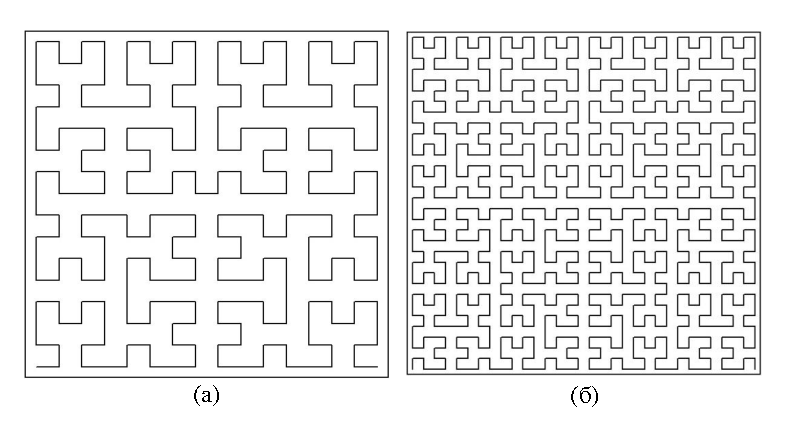
\includegraphics[scale=0.70]{figures/peano.pdf}}
%	\caption{Отображение отрезка $[0,1]$ с плотностью развертки: (а) $p=4$, (б) $p=5$}
%	\label{fig_peano}
%\end{figure}

Известно, что схема редукции размерности с использованием кривых Пеано сопоставляет многомерной задаче с липшицевой целевой функцией (\ref{eq1}) задачу (\ref{eq2}) с одномерной целевой функцией, удовлетворяющей условию Гёльдера
\begin{equation}\label{eq4} 
| f(x')-f(x'') | \leq K \rho(x',x''), \; x',x'' \in [0,1],
\end{equation}
где $\rho(x',x'') =  |x' - x''|^{1/N}$ -- метрика Гёльдера, $N$ -- размерность исходной задачи, а коэффициент $K$ связан с константой Липшица $L$ соотношением $K \leq 2L\sqrt {N+3}$ [\ref{rfa:rulit:Strongin2000}].

\section{Алгоритм решения задач с частично определенной целевой функцией}\label{alg_discr}

Алгоритм глобального поиска предполагает построение последовательности точек \textit{поисковых испытаний} $y^i \in D$, в которых вычисляются значения целевой функции $z^i = \varphi(y^i)$. Согласно используемой схеме редукции размерности, проведение испытания предполагает вычисление значения $y^i=y(x^i), x^i \in [0,1]$. При этом каждой точке испытания $x^i$ ставится в соответствие индекс $v^i$, определяемый по правилу
\begin{equation}\label{eq6} 
v(x^i) =
  \begin{cases}
    -1, & {\quad \text{если } x^i \text{ -- граничная точка}},\\
    0, & {\quad \text{если } x^i \text{ -- невычислимая точка}},\\
    1, & {\quad \text{если } x^i \text{ -- внутренняя точка}}.
  \end{cases}
\end{equation}

Результатом испытания является набор значений $(x^i, y^i=y(x^i), z^i = \varphi(y^i), v^i = v(x^i))$. 

Накопленная после проведения $k$ испытаний поисковая информация хранится в порядке возрастания значений координаты $x^i$ в множестве $\Omega_k$, в котором соответствующие записи для удобства перенумерованы нижним индексом.

На каждом шаге алгоритма производится вычисление оценки константы Гёльдера, определение характеристик поисковых интервалов, выбор наиболее перспективного интервала и вычисление точки $y^{k+1}$ для проведения очередного испытания.
Правила вычисления характеристики интервала для задач с частично определенной целевой функцией представлены в виде Алгоритма \ref{charact_alg}. 
%Сходимость метода в этом случае требует доказательства, которое будет продемонстировано авторами в будущих статьях.


%\begin{algorithm}
%\caption{Алгоритм оценки константы Гёльдера }\label{mu_alg}
%\begin{algorithmic}[1]
%\Require $\Omega_k$
%\Ensure $M$
%\State $M \gets \max\left\{ \frac{|z_i-z_{i-1}|}{\Delta _i},\quad v(x_{i-1}) = 1 \text{ and } v(x_i) = 1, \quad 1 \leq i \leq k  \right\}$
%    \If {$M = 0$}
%       \State $M = 1$
%   \EndIf\\
%\Return M
%\end{algorithmic}
%\end{algorithm}

\begin{algorithm}
\caption{Вычисление характеристики $i$-го интервала}\label{charact_alg}
\begin{algorithmic}[1]
\Require $\Omega_k, i, z^*, \mu, r >1, 0 < \alpha \leq 1$
\Ensure $R$

\If {$v(x_{i-1}) = 1 \text{ and } v(x_{i}) = 1$}  \Comment{ обе точки являются внутренними }
           \State $R \gets \Delta _i+\frac {{(z_i-z_{i-1})}^2}{{(r \mu)}^2 \Delta _i} - 2 \frac {(z_i+z_{i-1}-2z^*)}{r \mu}$
\ElsIf {$v(x_{i}) = 1$}  \Comment{ точка $x_i$ является внутренней }
           \State $R \gets 2 \Delta _i-4 \frac {(z_i-z^*)}{r \mu}$
\ElsIf {$v(x_{i-1}) = 1$} \Comment{ точка $x_{i-1}$ является внутренней }
            \State $ R \gets 2 \Delta _i-4 \frac {(z_{i-1}-z^*)}{r \mu}$
\Else \Comment{ обе точки являются невычислимыми или граничными }
           \State $R \gets \alpha{(1-\frac{1}{r})}^2 \Delta _i$
\EndIf\\
\Return R
\end{algorithmic}
\end{algorithm}

Значения $r$ и $\alpha$ являются параметрами алгоритма (их смысл пояснен ниже), а $\Delta_i$ обозначает длину $i$-го интервала в новой метрике,
\[
\Delta _i= (x_i-x_{i-1})^{1/N}.
\]

Подробное описание правил алгоритма глобального поиска на случай не всюду вычислимой целевой функции для решения задачи (\ref{eq2}) приведено в виде Алгоритма \ref{main_alg}.

\begin{algorithm}
\caption{Алгоритм глобального поиска для не всюду вычислимой целевой функции (АГП-Н)}\label{main_alg}
\begin{algorithmic}[1]
\Require $\varphi(y), D, \varepsilon, K_{max}, r >1, 0 < \alpha \leq 1$
\Ensure $y^{min}$
\State $\Omega_k \gets \left\{(x^1 = 0.0, y^1 = y(x^1), v^1=v(x^1)), (x^2 = 1.0, y^2 = y(x^2), v^2 = v(x^2))\right\}$
\State $\Omega_k \gets \Omega_k \cup \left\{(x^3 = 0.5, y^3 = y(x^3), z^3 = \varphi(y^3), v^3 = v(x^3))\right\}$
\State $z^* \gets z^3; k \gets 3; t \gets 2$
\While{ $\Delta_t \geq \varepsilon \text{ and } k \leq K_{max} \text{ or } v(x_t) \neq 1 \text{ and } v(x_{t-1}) \neq 1 $}
    \State $\mu \gets \max\left\{ \frac{|z_i-z_{i-1}|}{\Delta _i},\quad v(x_{i-1}) = 1 \text{ and } v(x_i) = 1, \quad 1 \leq i \leq k  \right\}$
    \If {$\mu = 0$}
       \State $\mu = 1$
   \EndIf
    \For{$i=1$ \textbf{to} $k$}
        \State $R_i \gets R(\Omega_k, i, z^*, \mu, r, \alpha)$
    \EndFor
    \State $t \gets \min \left\{\arg\max \left\{ R_i, 1 \leq i \leq k \right\}\right\}$
     \If {$v(x_{t-1}) = 1 \text{ and } v(x_t) = 1$}
        \State $x^{k+1} \gets \frac {x_t+x_{t-1}}{2} -  \text{sign} {(z_t-z_{t-1})} \frac{1}{2r} \left[\frac {{|z_t-z_{t-1}|}}{\mu} \right]^N$
    \Else
        \State $x^{k+1} \gets \frac {x_t+x_{t-1}}{2}$
    \EndIf
    \State $y^{k + 1} \gets y(x^{k + 1}); z^{k + 1} \gets \varphi(y^{k + 1}); v^{k+1} \gets v(x^{k+1})$
    \State $z^* = \min \left \{z^*, z^{k+1}\right \}$
    \State$\Omega_k \gets \Omega_k \cup \left\{(x^{k+1}, y^{k+1}, z^{k+1}, v^{k+1})\right\}$
    \State $k \gets k + 1$
\EndWhile
\State $min \gets \arg \min \left\{ z^i, 1 < i < k \right\}$\\
\Return $y^{min}$
\end{algorithmic}
\end{algorithm}

\textbf{Замечание 1 (о связи с АГП)}. В случаях, когда задача не содержит скрытых ограничений или проводимые алгоритмом испытания не попадают в существующие области невычислимости, АГП-Н полностью повторяет работу своего прототипа -- алгоритма глобального поиска.

\textbf{Замечание 2 (о параметре $\alpha$)}. Параметр $0 < \alpha \leq 1.0$ позволяет регулировать плотность сетки испытаний в области невычислимости $I$, $I \subset D$. Чем меньше параметр, тем менее перспективными для алгоритма будут интервалы с граничными точками в областях невычислимости. При максимально допустимом параметре $\alpha = 1.0$ метод густо усеивает точками испытаний подобласти, в которых функция не вычислима, возникает эффект <<черного пятна>> (точки испытаний в таких подобластях на рисунке обозначены черным цветом), см. Рис. \ref{task_61}a и Рис. \ref{task_61}б. При уменьшении параметра $\alpha$ точек этих испытаний становится значительно меньше, что наглядно видно на Рис. \ref{task_61}в и Рис. \ref{task_61}г.

\begin{figure}[h!]
	\center{\includegraphics[scale=0.15]{figures/task_61.png}}
	\caption{Распределение точек испытаний с различными видами невычислимых областей и настройкой параметра $\alpha$: (а) область невычислимости на границе области поиска, $\alpha = 1.0$; (б) случайно расположенные области невычислимости, $\alpha = 1.0$; (в) область невычислимости на границе области поиска, $\alpha = 0.08$; (г) случайно расположенные области невычислимости, $\alpha = 0.08$}
	\label{task_61}
\end{figure}

\textbf{Замечание 3 (о существовании вычислимого отрезка на кривой Пеано)}. В случае попадания точек испытаний в область невычислимости на первых итерациях, алгоритм будет выбирать лучший интервал на основе длин интервалов (т.е. будет строится равномерная сетка). Так как мы предполагаем, что область вычислимости целевой функции $Q = D \backslash I$ -- положительного объёма, то последующее сгущение сетки приведет к попаданию очередной точки испытания в область $Q$.

%\begin{figure}[h!]
%	\center{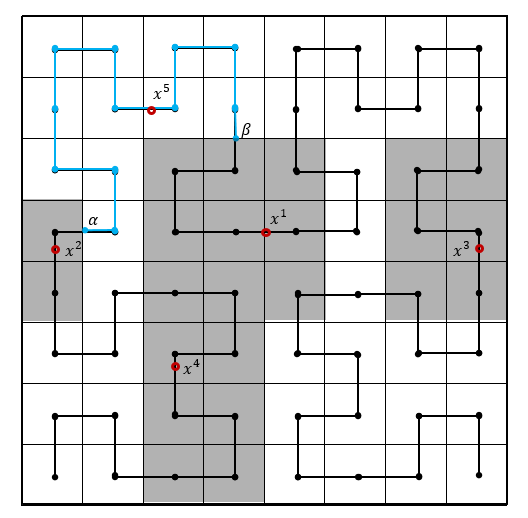
\includegraphics[scale=0.30]{figures/fig_0.png}}
%	\caption{Пример расстановки точек испытаний до момента попадания в вычислимую точку}
%	\label{fig_1}
%\end{figure}


\textbf{Замечание 4 (о решении задач с дискретными параметрами)}. Алгоритм глобального поиска допускает обобщение для решения задач, в которых часть переменных являются непрерывными, а часть может принимать только дискретные значения [\ref{rfa:rulit:Barkalov2021}]. Это позволяет применять АГП-Н в задачах, где часть параметров объекта оптимизации может принадлежать некоторому дискретному множеству. Подобные задачи часто возникают при настройке гиперпараметров методов машинного обучения.

\section{Программная реализация} \label{iOpt_discr}

Алгоритм глобального поиска, предназначенный для решения задач с не всюду вычислимой целевой функцией (АГП-Н), был реализован на базе открытого фреймворка методов интеллектуальной оптимизации iOpt [\ref{rfa:rulit:iOptPaper},\ref{rfa:rulit:iOptGithub}]
%с открытым исходным кодом [\ref{rfa:rulit:iOptGithub}].

\begin{figure}[h!]
	\center{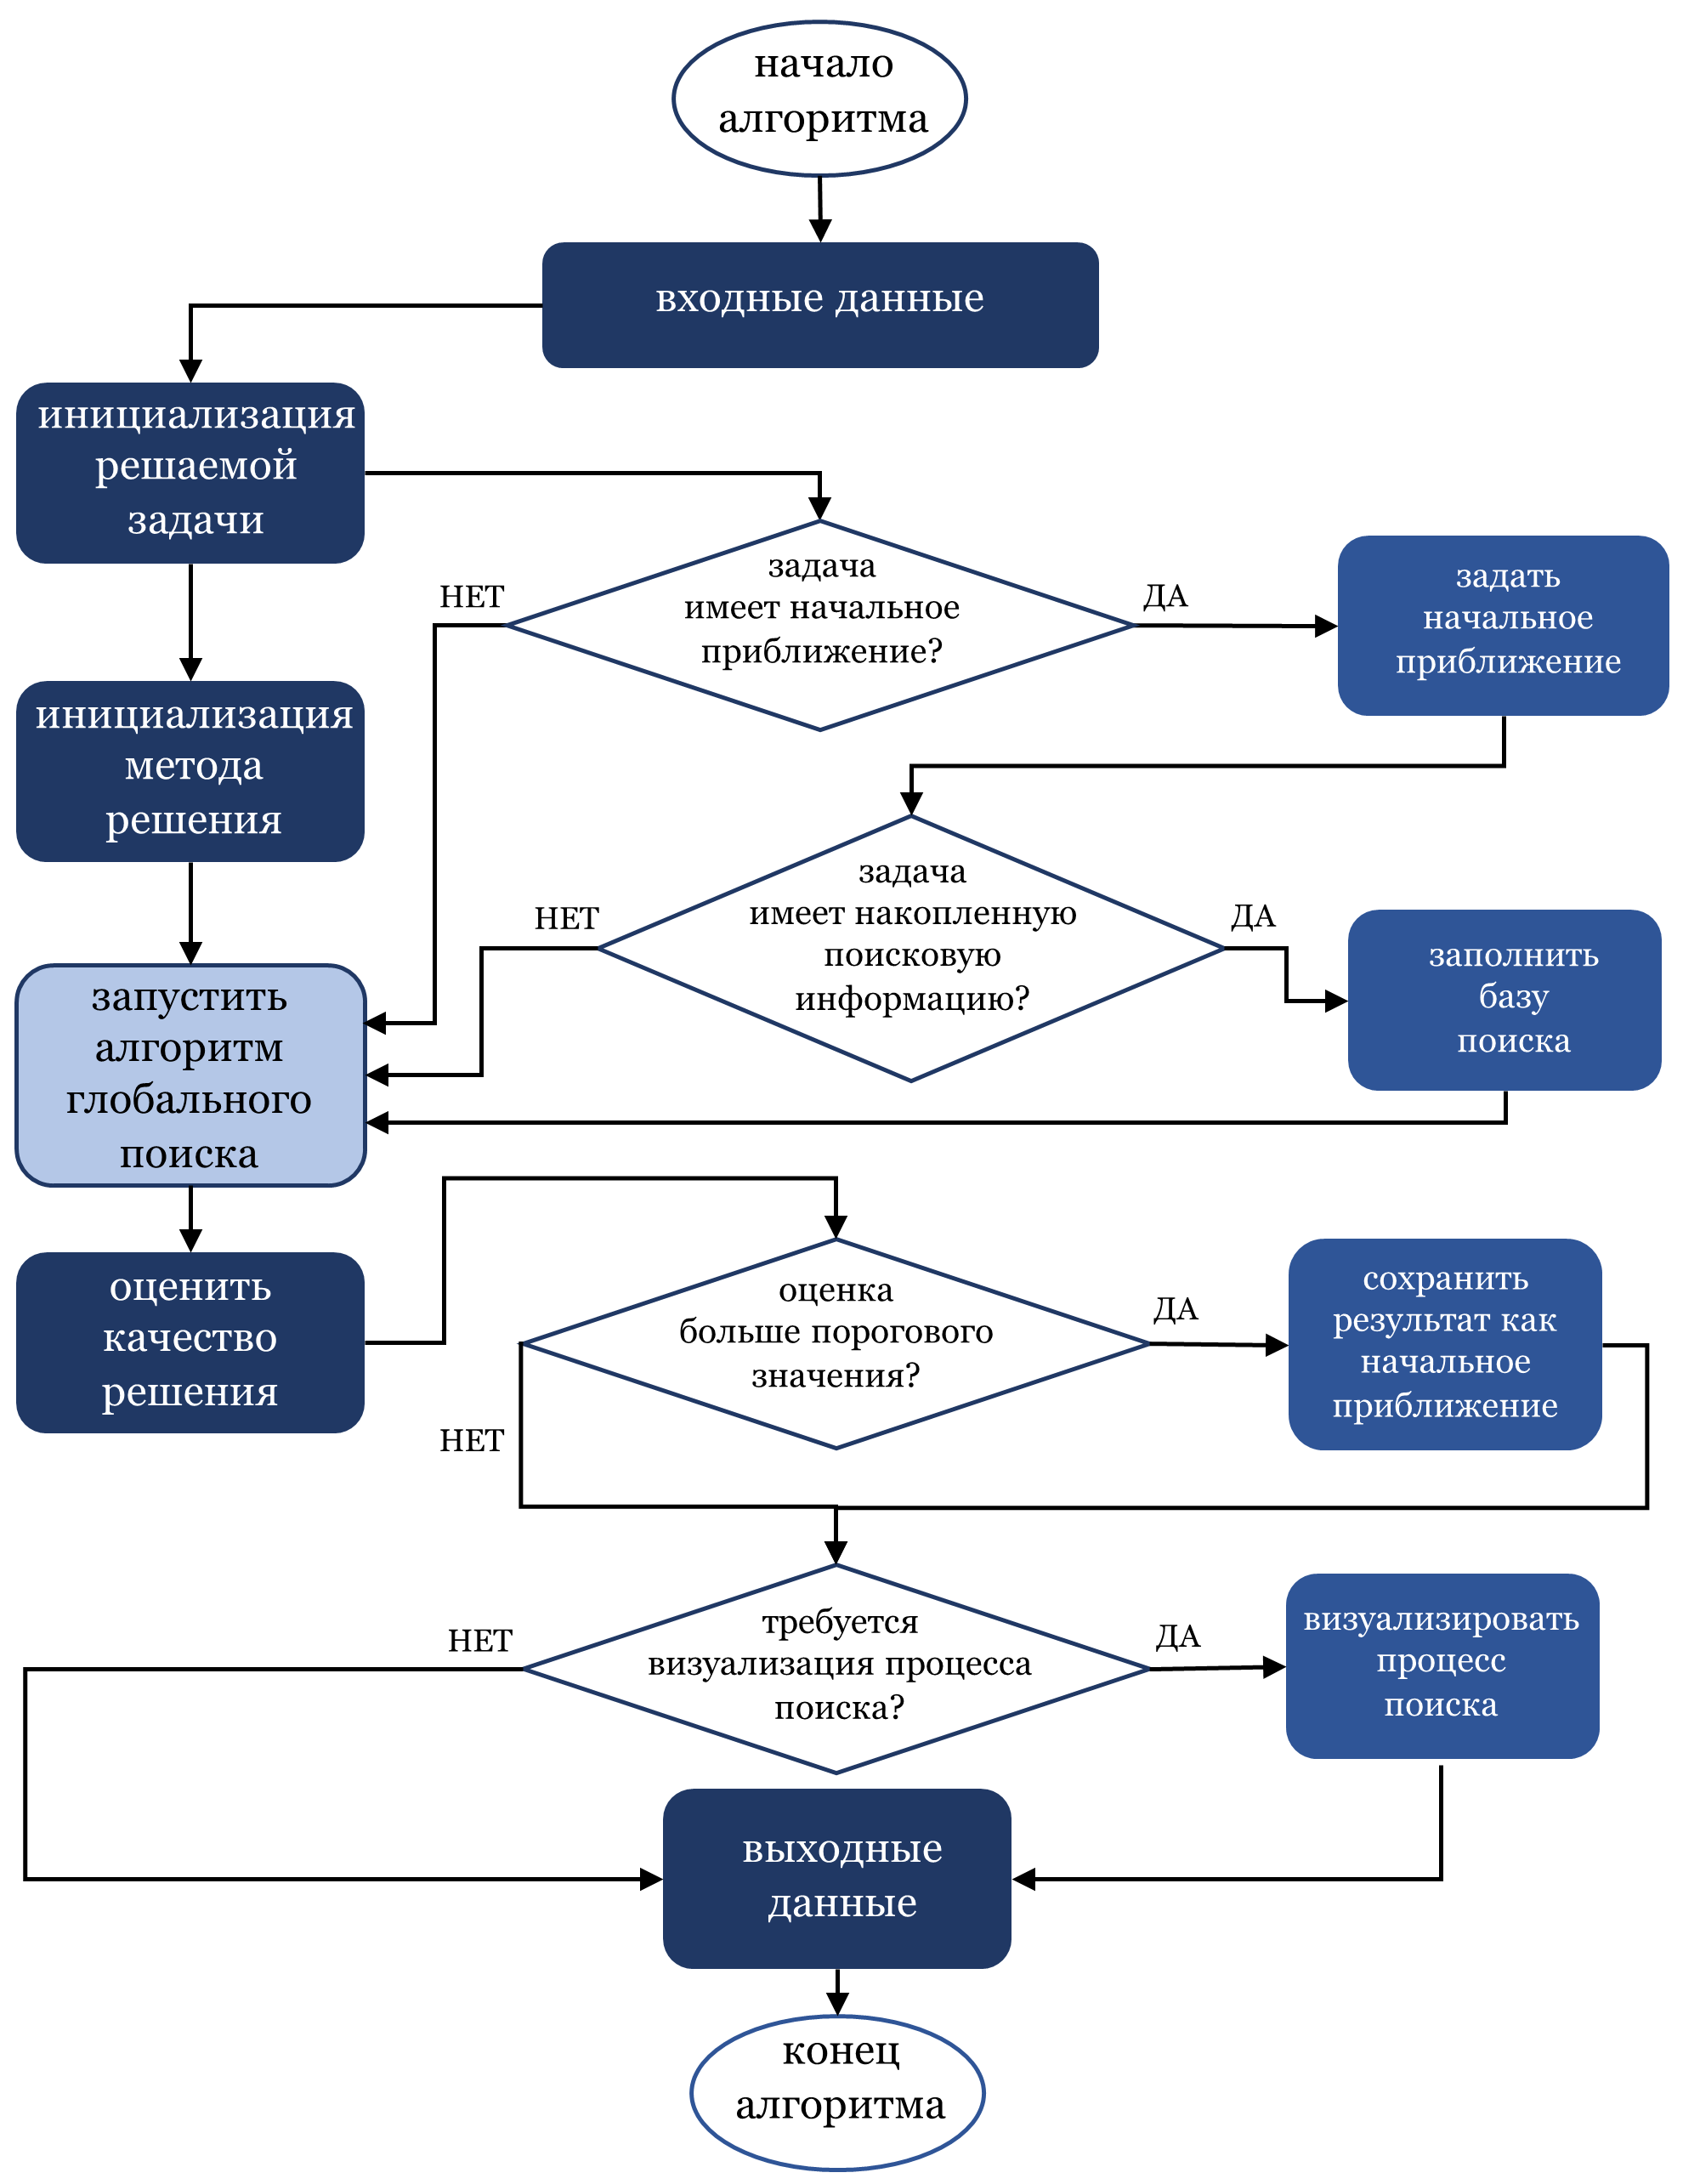
\includegraphics[scale=0.82]{sheme.png}}
	\caption{Блок-схема общего алгоритма функционирования фреймворка iOpt}
	\label{fig_iOpt}
\end{figure}

Фреймворк позволяет проводить точную настройку параметров моделей и методов, используемых в прикладных исследованиях в различных научных областях. Характерными примерами задач, решаемых фреймворком iOpt, являются задачи настройки гиперпараметров методов машинного обучения. В таких задачах часто возникает рассматриваемая в данном исследовании проблема частичной определенности критериев в отсутствии формульного описания исследуемой модели вида <<черный ящик>>. 

На Рис.~\ref{fig_iOpt} приведена блок-схема общего алгоритма функционирования фреймворка.

Фреймворк iOpt написан на Python в виде системы взаимосвязанных классов. Реализация описанного в разделе \ref{alg_discr} алгоритма содержится в базовом классе Method. Описанный далее в разделе \ref{GKLS_HC} генератор задач GKLS со скрытыми ограничениями (GKLS-HC) реализован в виде класса GKLSHiddenConstraint -- наследника интерфейса Problem. В фреймворк добавлена возможность визуализации процесса решения задач со скрытыми ограничениями с использованием StaticPainterNDListener. Доступны различные способы отрисовки линий уровня целевой функции: по равномерной сетке, только по точкам поисковых испытаний, по точкам испытаний с использованием интерполяции. Подробное описание возможностей фреймворка представлено в документации [\ref{rfa:rulit:iOptDocs}].

\section{Результаты вычислительных экспериментов}

\subsection{Решение серий тестовых задач} \label{GKLS_HC}

Решение серии задач с известными свойствами является одним из традиционных способов оценки качества работы методов глобального поиска. 
Однако доступные наборы тестовых задач не содержат областей невычислимости целевой функции, поэтому для тестирования разработанного алгоритма АГП-Н был предложен способ генерации тестовых задач со скрытыми ограничениями.

В данном разделе дано краткое описание тестовых задач, а также приведены результаты экспериментов, демонстрирующие надёжность глобального поиска и эффективность разработанного алгоритма оптимизации.

\subsubsection{Описание тестовых задач} \label{GKLS_HC}
 
Для создания тестовых задач GKLS-HC использовался генератор GKLS [\ref{rfa:rulit:Gaviano2003}], позволяющий порождать задачи многоэкстремальной оптимизации с заранее известными свойствами. 

Генерация задачи состоит в определении выпуклой квадратичной функции, дополненной полиномами более высокого порядка для введения локальных минимумов. Каждый тестовый класс, предоставляемый генератором GKLS, состоит из 100 функций, построенных случайным образом, и определяется размером области поиска, количеством локальных минимумов, значением глобального минимума, радиусом области притяжения глобального минимума, расстоянием от глобального минимума до вершины квадратичной функции. Другие необходимые параметры, такие как точки всех локальных минимумов, их области притяжения и значения, выбираются генератором случайным образом.

Данные функции были дополнены областями невычислимости в форме эллипсоидов (координаты центров и длины радиусов генерировались случайно), при попадании в которые функция возвращает исключение, сообщающее о невозможности вычислить ее значение.

В текущей версии фреймворк iOpt использует генератор GKLS для формирования задач с размерностью от 2 до 5, числом локальных минимумов равным 10 и областью поиска от $-1$ до $1$ по каждой переменной. Радиус области притяжения глобального минимума и расстояние от глобального минимума до вершины квадратичной функции варьируется в зависимости от размерности задачи. Количество генерируемых областей невычислимости задавалось равным 4. Области невычислимости могут пересекаться, при этом не включают точку известного глобального минимума функций GKLS по построению. Радиусы областей невычислимости выбираются случайно из диапазона $[0.05, 0.25]$.

Если говорить о программной реализации, то генератор задач реализован в виде класса GKLSHiddenConstraint, конструктор которого принимает размерность генерируемой задачи (от 2 до 5), номер функции (от 1 до 100), а также параметр для настройки генератора случайных чисел для воспроизведения экспериментов, после чего автоматически устанавливает остальные параметры генератора.

\subsubsection{Результаты решения тестовых задач с помощью АГП-Н}

Вычислительный эксперимент был проведен с использованием фреймворка iOpt, описанного в разделе \ref{iOpt_discr}. АГП-Н запускался на серии задач GKLS-HC с точностью поиска минимума $\varepsilon = 0.001$, параметром надёжности $r = 4.2$ и двумя значениями параметра $\alpha$: $\alpha = 0.08$ и $\alpha = 0.008$. Для полноценного сравнения алгоритм АГП-Н также был запущен на серии задач GKSL (т.е. на задачах без подобластей, в которых целевая функция является неопределенной), что соответствует поведению исходного АГП.

Результаты эксперимента приведены в таблице \ref{iOpt_gkls}.

На Рис. \ref{oper_charact} показаны операционные характеристики, которые демонстрируют для каждого количества итераций число задач из тестовой выборки, решенное с заданной точностью $\varepsilon = 0.001$. 

\begin{table}[h!]
\centering
\caption{Результаты решения задач GKLS и GKLS-HC средствами фреймворка iOpt}
\begin{tabular}{|r|c|c|}
\hline
 класс задач & $\alpha$ & среднее число итераций \\ \hline\hline
\multirow{2}{*}{GKLS-HC} & 0.08 & 2151 \\ \cline{2-3} 
 & 0.008 & 1635 \\ \hline
GKLS & - & 1510 \\ \hline
\end{tabular}
\label{iOpt_gkls}
\end{table}

\begin{figure}[h!]
	\center{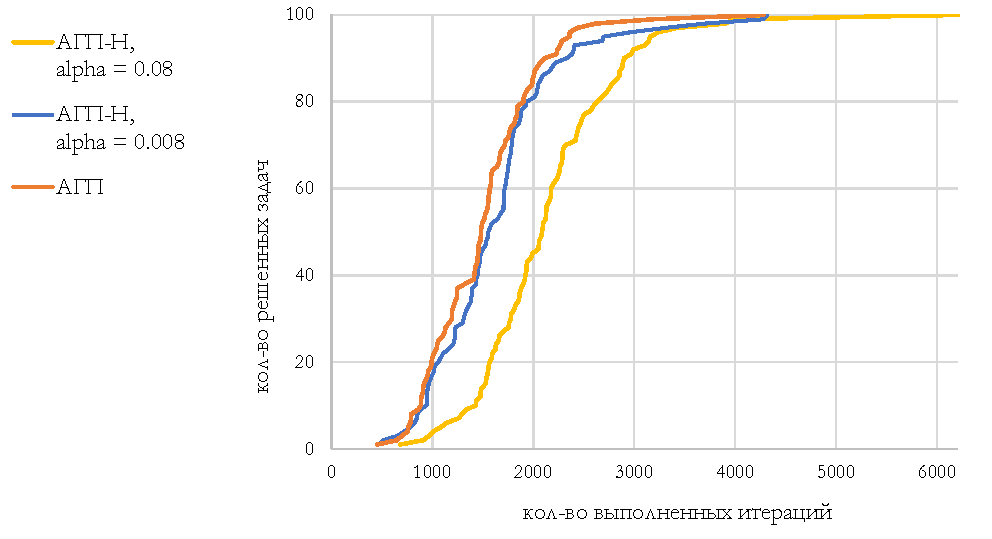
\includegraphics[scale=0.9]{figures/oper_charact_transp.pdf}}
	\caption{Операционные характеристики алгоритмов АГП-Н и АГП}
	\label{oper_charact}
\end{figure}

%\begin{table}[h!]
%\centering
%\caption{Результаты решения задач GKLS и GKLS-HC средствами фреймворка iOpt}
%\begin{tabular}{||r|c|c|c||}
%\hline
%\multicolumn{1}{||c|}{} & alpha & \begin{tabular}[c]{@{}c@{}}среднее\\ число\\ итераций\end{tabular} & \begin{tabular}[c]{@{}c@{}}кол-во\%\ решенных\\ задач\end{tabular} \\ \hline
%\multirow{2}{*}{GKLS-HC} & 0.08  & 2151 & 100 / 100 \\ \cline{2-4} 
%                                        & 0.008 & 1635 & 100 / 100 \\ \hline
%GKLS                                    & -     & 1510 & 100 / 100 \\ \hline
%\end{tabular}
%\label{iOpt_gkls}
%\end{table}

Примеры визуализации процесса решения задачи GKLS-HC №~38 представлены на Рис. \ref{iOpt_result}. Черными точками отмечены точки испытаний, попавшие в подобласти неопределенности функции. Красной точкой отмечено найденное алгоритмом решение.

\begin{figure}[h!]
	\center{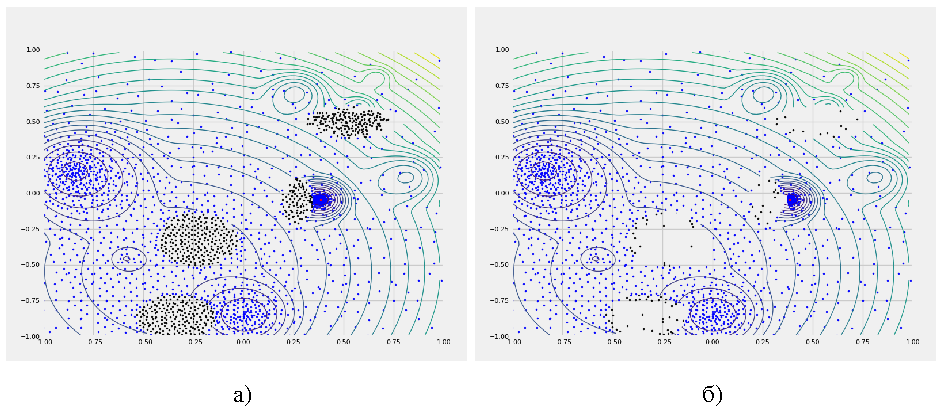
\includegraphics[scale=1]{figures/iOpt_result.pdf}}
	\caption{Графики линий уровня задачи GKLS-HC №~38 с точками проводимых испытаний, полученные средствами фреймворка iOpt: (а) $\alpha = 0.08$, (б) $\alpha = 0.008$ }
	\label{iOpt_result}
\end{figure}

Результаты проведенных экспериментов показывают, что после выполнения 2000 итераций АГП-Н с параметром $\alpha = 0.008$ будет получена оценка оптимума с требуемой точностью для 80\% задач. Для решения оставшихся 20\% задач требуется (в худшем случае) 4315 поисковых испытаний. Отметим, что за счёт регулировки параметра $\alpha$ получилось добиться такой же скорости работы, как у  АГП при решении серии задач GKLS (в терминах числа испытаний, требующихся для решения задач с заданной точностью).

\subsection{Сравнение АГП-Н с известными алгоритмами оптимизации}

АГП-Н может быть использован не только в задаче настройки гиперараметров различных методов, но и для решения рядовых оптимизационных задач из различных прикладных областей. В связи с этим имеет смысл привести сравнение реализованного метода с существующими оптимизаторами на задачах с не всюду вычислимой целевой функцией.

\subsubsection{Описание алгоритмов оптимизации}

В данной статье сравнение проводилось с алгоритмами глобальной оптимизации библиотеки \textit{scipy.optimize}, а именно с методами \textit{differential\_evolution} [\ref{rfa:rulit:differential_evolution}], \textit{dual\_annealing} [\ref{rfa:rulit:dual_annealing}], \textit{direct} [\ref{rfa:rulit:direct}], \textit{basinhopping} [\ref{rfa:rulit:basinhopping}], \textit{shgo} [\ref{rfa:rulit:shgo}], \textit{brute}.

Метод дифференциальной эволюции (differential evolution) -- один из самых известных генетических алгоритмов вещественной оптимизации. Во многих практических задачах метод обеспечивает приемлемое решение, т.к. не использует информацию о градиенте функции, а схемы мутации и рекомбинации позволяют ему <<выходить>> из локальных минимумов.

Двойной отжиг (dual annealing) -- алгоритм глобальной оптимизации, основанный на комбинировании алгоритмов классического и быстрого имитационного отжига. Алгоритм имитирует процесс отжига в металлургии. Отжиг заключается в нагревании и контролируемом охлаждении металла для формирования устойчивой кристаллической решётки: при высокой температуре системы алгоритм использует более широкий диапазон решений, при снижении температуры диапазон поиска становится всё меньше, пока не будет найден глобальный оптимум.

Direct (DIviding RECTangles), как и АГП, предназначен для решения задач липшицевой глобальной оптимизации. Особенностью метода является отказ от оценивания константы Липшица. В процессе своей работы алгоритм разбивает область поиска на гиперинтервалы, среди которых выбираются потенциально оптимальные (подлежащие дальнейшему разбиению), после чего в их центрах проводится вычисление значений целевой функции.

Перепрыгивание через бассейн (basin-hopping) -- алгоритм глобальной оптимизации, осуществляющий поиск оптимума путём последовательного выполнения локальной оптимизации (по умолчанию используя метод Монте-Карло) с последующим принятием или отклонением новых координат на основе текущего лучшего значения функции.

SHGO (simplicial homology global optimization) -- сравнительно новый алгоритм глобальной оптимизации, основанный на применении симплициальной гомологии. Алгоритм использует концепции из комбинаторной интегральной теории гомологии для поиска подобластей, которые приблизительно локально выпуклы. В отличие от многих других алгоритмов глобальной оптимизации, использующих теорию графов и методы кластеризации, SHGO создает начальные точки, которые сходятся к уникальным локальным минимумам, что улучшает его производительность.

Метод brute реализует метод <<грубой силы>> (brute force), т.е. полный перебор.

Алгоритмы \textit{differential\_evolution}, \textit{dual\_annealing}, \textit{basinhopping} относятся к классу стохастических алгоритмов (т.е. каждый запуск поиска может найти другое решение), потому поиск глобального минимума с использованием данных алгоритмов требует многократных запусков.

\subsubsection{Результаты проведенного сравнения}

В рамках проведенного эксперимента были получены следующие результаты.

При наличии у задачи скрытых ограничений худшее поведение демонстрируют алгоритмы \textit{differential\_evolution} и \textit{brute}. Алгоритм \textit{differential\_evolution} полностью исчерпывает все выделенные ему итерации, не находя при этом корректный ответ. Полный перебор в свою очередь в качестве результата работы может вернуть что угодно. 

Алгоритмы \textit{dual\_annealing} и \textit{basinhopping} в ряде случаев справляются с поставленной оптимизационной задачей. При этом в рамках эксперимента количество вычислений целевой функции алгоритмом \textit{dual\_annealing} составило порядка 4000, в то время как \textit{basinhopping} мог выполнять и 140000 вычислений для одной задачи.

Алгоритмы \textit{direct} и \textit{shgo} демонстрируют хорошие результаты, хоть и не всегда обладают сходимостью. Среднее число итераций алгоритма \textit{direct} составило 94 (соответствует 1981 вычислениям целевой функции). Алгоритм \textit{shgo} в каждой задаче полностью исчерпал выделенные ему 200 итерации, выполняя в среднем 4482 вычислений целевой функции. В сравнении с данными методами АГП-Н работает эффективнее (отметим, что одна итерация АГП-Н соответствует одному вычислению значения целевой функции) и обладает лучшей сходимостью к глобальному оптимуму.

\begin{table}[h!]
\centering
\caption{Возможные выявленные результаты работы алгоритмов глобальной оптимизации библиотеки \textit{scipy.optimize} на задачах GKLS-HC}
\begin{tabular}{|r|c|c|c|c|}
\hline
\multirow{2}{*}{алгоритм} & \multicolumn{4}{c|}{возможный результат поиска} \\ \cline{2-5} 
 & \multicolumn{1}{c|}{глобальный минимум} & \multicolumn{1}{c|}{локальный минимум} & \multicolumn{1}{c|}{nan} & \multicolumn{1}{c|}{1e+100} \\ \hline\hline
АГП-Н                   &     \CIRCLE   &                   &              &             \\ \hline
differential\_evolution &                    &                   &  \CIRCLE  &             \\ \hline
dual\_annealing         &     \CIRCLE     &                   &  \CIRCLE  &             \\ \hline
basinhopping            &     \CIRCLE     &    \CIRCLE    &              &  \CIRCLE \\ \hline
direct                  &     \CIRCLE    &    \CIRCLE     &              &             \\ \hline
shgo                    &     \CIRCLE     &    \CIRCLE     &              &             \\ \hline
brute                   &     \CIRCLE     &    \CIRCLE    &  \CIRCLE  &  \CIRCLE \\ \hline
\end{tabular}
\label{comparision}
\end{table}

В таблице \ref{comparision} собрана информация о возможном поведении исследованных алгоритмов с задачами с не всюду определенной целевой функцией, обнаруженная при решении задач GKLS-HC. Алгоритм АГП-Н всегда находит глобальный минимум, тогда как differential\_evolution всегда возвращает значение nan. Остальные алгоритмы могут вернуть как глобальный, так и локальный минимум, при этом алгоритмы dual\_annealing и basinhopping в ряде случаев могут вернуть значения nan и 1e+100 соответственно, а алгоритм brute, как уже было отмечено, и вовсе может вернуть в качестве ответа что угодно.

\subsection{Решение задач настройки методов машинного обучения}

\subsubsection{Настройка гиперпараметров метода LinearSVC}

В качестве первой модельной задачи оптимизации, в которой встречается недопустимое сочетание параметров, рассмотрим настройку гиперпараметров метода LinearSVC из библиотеки \textit{scikit-learn} при решении задачи классификации. 

Исследование проводилось на классическом датасете Iris, который содержит характеристики трех различных видов ириса и часто используется в качестве тестового примера для алгоритмов машинного обучения. Набор данных Iris состоит из 150 записей (по 50 записей на каждый вид ириса), содержащих по 5 атрибутов. Датасет включен в библиотеку машинного обучения \textit{scikit-learn}.

Задача заключалась в максимизации метрики $F1$, характеризующей качество построения классификатора. Для LinearSVC варьировались 2 дискретных и 1 непрерывный параметры:
\begin{itemize}
\item[--] тип функции потерь $loss$, $loss \in \{hinge, squared\_hinge\}$;
\item[--] параметр $dual$, $dual \in \{true, false\}$, который позволяет выбирать между решением двойственной или основной задачи оптимизации;
\item[--] коэффициент регуляризации $C$, $C \in [1,6]$.
\end{itemize}
Для возможности воспроизведения результатов параметр $random\_state$ был зафиксирован в значении 10. Остальные параметры метода LinearSVC рассматривались заданными по умолчанию.

Отметим, что сочетание гиперпараметров $loss = hingle$ и $dual = False$ приводит к <<падению>> метода LinearSVC (метод выбрасывает исключение и не выдает значения целевой метрики).

Поставленная задача решалась в области изменения гиперпараметров с использованием следующих алгоритмов:
\begin{itemize}
\item[--] АГП-Н (предложенный в данной статье) с использованием параметра надежности $r=3.5$ и ограничением на число испытаний $K_{max}=100$;
\item[--] GridSearchCV (метод полного перебора по равномерной сетке);
\item[--] RandomizedSearchCV (метод случайного поиска).
\end{itemize}
 
Полученные результаты представлены в таблице \ref{tab22}. Отметим, что в процессе своей работы оба алгоритма библиотеки \textit{scikit-learn} решили задачу с выдачей предупреждения о возникновении недопустимого сочетания параметров. Алгоритм АГП-Н нашел лучшее значение $F1 = 0.973$ при сочетании значений гиперпараметров $C=1.3125$, $loss=squared\_hinge$, $dual = False$.

\begin{table}[h!]
\centering
\caption{Результаты настройки гиперпараметров метода LinearSVC при решении задачи классификации на датасете Iris}\label{tab22}
\begin{tabular}{|r|c|c|}
\hline
метод & финальная F1 \\
\hline \hline
АГП-Н & 0.973 \\
\hline
GridSearchCV & 0.96 \\
\hline
RandomizedSearchCV & 0.96 \\
\hline
\end{tabular}
\end{table}

%%%%% new

\subsubsection{Настройка гиперпараметров метода предсказания значений временного ряда }

В качестве второй модельной задачи рассмотрим задачу настройки гиперпараметров методов предсказания значений временного ряда (time series forecasting). Предсказание значений производилось с использованием фреймворка FEDOT [\ref{nikitin2022automated}]
(фреймворк с открытым исходным кодом для задач автоматизированного моделирования и машинного обучения, AutoML). FEDOT поддерживает полный цикл решения задачи, включающий препроцессинг, выбор модели, настройку, кроссвалидацию и т.д. Фреймворк использует ML-модели, в основном из стандартных библиотек \textit{sklearn}, \textit{statsmodels} и \textit{keras}.

Исследование проводилось на датасете \textit{montly beer production}, который содержит 476 записей. %\cite{MonthlyBeerDataset,MonthlyBeerArticle}
Указанный датасет представлен на платформе Kaggle и часто используется для тестирования алгоритмов машинного обучения (см., например, [\ref{MonthlyBeerArticle}]).
Построенный для решения поставленной задачи в FEDOT пайплайн включает в себя комбинацию из двух преобразований: lagged и cgru. Lagged-преобразование выполняется путем взятия значения переменной в предыдущий момент времени и включения его в модель в качестве признака в текущий момент времени. Для этого данные временного ряда сдвигаются на определенное количество шагов, которые называются лагом или временной задержкой. В качестве используемой нейронной сети выступает рекуррентная сеть (GRU), использующая свертку (CGRU).

%%%% КАРТИНКА ПОД ВОПРОСОМ
%\begin{figure}[h!]
%\center
%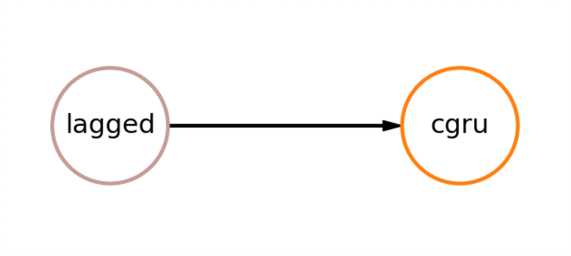
\includegraphics[width=0.4\textwidth]{fig2.png}
%\caption{Визуализация пайплайна с простейшей схемой архитектуры сети CGRU.} \label{fig2}
%\end{figure}

У lagged-преобразования имеется один параметр window\_size, который изменяется от 5 до 250 с шагом 1. Поскольку этот параметр имеет большое количество значений, при оптимизации, будем рассматривать его как непрерывный (с округлением до единиц). У CGRU варьировались 4 дискретных и 2 непрерывных параметра:
\begin{itemize}
\item[--] cnn1\_kernel\_size $\in \{4, 5\}$,
\item[--] cnn2\_kernel\_size $\in \{5, 6\}$, 
\item[--] cnn1\_output\_size $\in \{32, 64\}$, 
\item[--] cnn2\_output\_size $\in \{32, 64\}$;
\item[--] hidden\_size $\in [20, 200]$, 
\item[--] learning\_rate $\in [0.0005, 0.005]$.
\end{itemize}
Остальные параметры были зафиксированы в значениях по умолчанию: batch\_size = 64, num\_epochs = 50, optimizer = 'adamw', loss = 'mse'.

Таким образом, фреймворк iOpt решал задачу минимизации метрики $MSE$, варьируя 3 непрерывных и 4 дискретных параметра, каждый из которых принимал 2 значения (всего 16 комбинаций). Отметим, что при некоторых сочетаниях параметров window\_size, cnn1\_kernel\_size, cnn1\_output\_size, cnn2\_kernel\_size и cnn2\_output\_size невозможно вычислить значение критерия (метод возвращает бесконечное значение функции). Такие точки рассматривались как невычислимые.

Для сравнения поставленная задача также была решена при помощи известного фреймворка оптимизации гиперпараметров Optuna%\cite{OptunaURL,optuna}
. Оба решателя были интегрированы в FEDOT и задействованы в вычислительном эксперименте.

Для решения поставленной задачи было выставлено ограничение на 1000 поисковых испытаний. В iOpt после 950 <<глобальных>> итераций глобального метода запускалось локальное уточнение с использованием метода Хука-Дживса. %%%%\cite{Himmelblau72}
Результаты проведенного эксперимента отражены в таблице~\ref{tab1}. 

\begin{table}[h!]
\centering
\caption{Результаты решения задачи настройки гиперпараметров метода предсказания значений временного ряда на датасете montly beer production с использованием фреймворков iOpt и Optuna}\label{tab1}
\begin{tabular}{|l|c|c|}
\hline
фреймворк & время решения, сек. & финальная MSE \\
\hline \hline
iOpt & 6574.2 & 13.5 \\
\hline
Optuna &  9554.1 & 13.4 \\
\hline
\end{tabular}
\end{table}

Число точек, в которых не получилось вычислить критерий оптимизации, составило порядка 10\% от общего числа точек поисковых испытаний. Кривые, соответствующие полученному предсказанию, приведены на Рис.~\ref{fig3}. Темная линия соответствует истинным значениям временного ряда, голубая -- предсказанным значениям, полученным после использования Optuna, желтая линия -- предсказанным значениям, полученным после использования iOpt.

\begin{figure}[h!]
\center 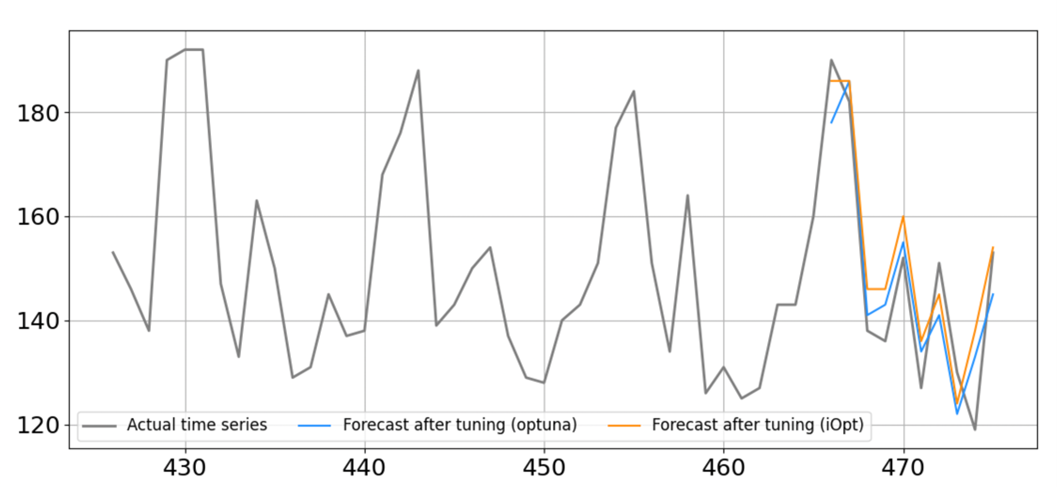
\includegraphics[scale=1.1]{fig3.png}
\caption{Визуализация предсказания и истинного значения временного ряда} \label{fig3}
\end{figure}

%%%%%% end new

\section{Заключение}

В настоящей работе рассматривалась актуальная проблема решения задач настройки гиперпараметров методов искусственного интеллекта (ИИ) и машинного обучения (МО).
Сложность таких задач заключается в большой трудоемкости оценки метрик качества методов ИИ и МО для заданного сочетания гиперпараметров, что ограничивает возможное число проверяемых комбинаций.
Одновременно с этим исследуемые методы ИИ и МО могут работать некорректно в некоторых заранее неизвестных подобластях всей области изменения гиперпараметров; фактически, область допустимых сочетаний гиперпараметров является неопределенной. Проблема возникновения некорректных сочетаний гиперпараметров, которая ранее не имела особого значения при <<ручной>> настройке, при использовании автоматической настройки стала весьма актуальной.

Для решения указанного класса задач была разработана модификация одного из эффективных детерминированных методов решения задач глобальной оптимизации -- ин\-фор\-ма\-ци\-он\-но-ста\-тис\-ти\-чес\-ко\-го алгоритма глобального поиска. Предложенный алгоритм глобального поиска для не всюду вычислимых функций (АГП-Н) реализован на базе фреймворка методов интеллектуальной оптимизации с открытым исходным кодом iOpt.

В статье подробно описаны вычислительные правила и приведена схема работы АГП-Н. Представлены результаты экспериментов на нескольких сотнях тестовых задач, демонстрирующие надежность предложенного подхода к обработке неопределенных значений оптимизируемой функции. Также приведены результаты сравнения работы АГП-Н и стандартных алгоритмов оптимизации из библиотеки SciPy, которые подтверждают эффективность разработанного метода при решении тестового класса задач.

В качестве модельных примеров были решены несколько задач настройки гиперпараметров, где возникает проблема возникновения недопустимых сочетаний гиперпараметров, при которых невозможно оценить целевую метрику качества.
В первом примере была проведена настройка гиперпараметров классического алгоритма классификации LinearSVC. АГП-Н успешно решил поставленную задачу, найдя лучшее сочетание гиперпараметров по сравнению со стандартными алгоритмами из библиотеки scikit-learn.
В качестве второй модельной задачи была рассмотрена настройка гиперпараметров метода предсказания значений временного ряда. В ходе эксперимента было проведено сравнение АГП-Н с алгоритмами настройки из широко известного фреймворка Optuna. АГП-Н показал сравнимый результат (в терминах полученного значения целевой метрики), значительно обогнав Optuna по времени, затраченному на решение задачи.



%В статье было приведено описание одной из исследованных ранее модификаций алгоритма глобального поиска для решения такого класса задач. Приведены теоретические обоснования сходимости алгоритма. Теоретические результаты полностью соответствуют картине, полученной в ходе экспериментальных исследований эффективности алгоритма. Разработанная модификация обладает недостатком в виде избыточных испытаний в области невычислимости (в силу порождения алгоритмом предельных точек в данных областях). Данного явления можно избежать с использованием более сложной модификации, восстанавливающей значения в невычислимых точках, основываясь на предположении о липшицевости целевой функции (что было отражено в экспериментальных исследованиях). Теоретическое обоснование данной модификации является объектом будущих исследований.

\textbf{Благодарности.} Работа выполнена при поддержке Министерства науки и высшего образования РФ (проект № FSWR-2023-0034) и научно-образовательного математического центра <<Математика технологий будущего>>.


\section*{Список литературы}
% оформленный в соответствии с требованиями ГОСТ
\begin{enumerate}
%7
%\item \label{rfa:rulit:Grishagin2016_2}
%Grishagin~V.A., Israfilov~R.A. Global search acceleration in the nested optimization scheme~// AIP Conference Proceedings. 2016. Vol. 1738. p. 400010. DOI: 10.1063/1.4952198.

\item \label{rfa:rulit:Zhou2021}
Zhou~J. , Qiu~Y.,  Zhu~S., Armaghani~D. J. , Li~C., Nguyen~H. , Yagiz~S. Optimization of support vector machine through the use of metaheuristic algorithms in forecasting {TBM} advance rate~// Engineering Applications of Artificial Intelligence. 2021. Vol.~97. p.~104015.  DOI: 10.1016/j.engappai.2020.104015.

\item \label{rfa:rulit:Yang2022}
Yang~W., Xia~K., Fan~S., Wang~L., Li~T., Zhang~J., Feng~Y. A Multi-Strategy Whale Optimization Algorithm and Its Application~// Eng. Appl. Artif. Intell. 2022. Vol.~108. p.~104558. DOI: 10.1016/j.engappai.2021.104558.

\item \label{rfa:rulit:Frazier2018}
Frazier~P.I. A Tutorial on Bayesian Optimization~// arXiv. 2018. DOI: 10.48550/arXiv.1807.02811.

\item \label{rfa:rulit:Archetti2019}
Archetti~F., Candelieri~A. Bayesian Optimization and Data Science. Cham: Springer Briefs in Optimization, 2019. DOI: 10.1007/978-3-030-24494-1.

%9
\item \label{rfa:rulit:Jones2021}
Jones~D., Martins~J. The direct algorithm: 25 years later~// J. Glob. Optim. 2021. Vol.~79, No.~3. P. 521--566. DOI: 10.1007/s10898-020-00952-6.

%12
\item \label{rfa:rulit:PaulaviciusZilinskas2014}
Paulavi{\v c}ius~R. and {\v Z}ilinskas~J. Simplicial Global Optimization. New York: Springer, 2014. DOI: 10.1007/978-1-4614-9093-7.

%13
\item \label{rfa:rulit:Birect2020}
Paulavi{\v c}ius~R., Sergeyev~Y.D., Kvasov~D.E., {\v Z}ilinskas~J. Globally-biased {BIRECT} algorithm with local accelerators for expensive global optimization~// Expert Syst. Appl. 2020. Vol.~144. p.~113052. DOI: 10.1016/j.eswa.2019.113052.

%14
\item \label{rfa:rulit:Sergeyev2017}
Сергеев~Я.Д., Квасов~Д.Е. Диагональные методы глобальной оптимизации.  М.: Физматлит, 2008. 

%11
\item \label{rfa:rulit:Liberti2005}
Liberti~L., Kucherenko~S. Comparison of deterministic and stochastic approaches to global optimization~// Int. Trans. Oper. Res. 2005. Vol.~12. P.~263--285.

%15
\item \label{rfa:rulit:Sergeyev2018}
Sergeyev~Y.D., Kvasov~D.E., Mukhametzhanov~M.S. On the efficiency of nature-inspired metaheuristics in expensive global optimization with limited budget~// Sci. Rep. 2018. Vol.~8, No.~1. p.~435.

%16
\item \label{rfa:rulit:Sergeyev2013}
Sergeyev~Y.D., Strongin~R.G., Lera~D. Introduction to Global Optimization Exploiting Space-Filling Curves. New York: Springer Briefs in Optimization, 2013. DOI: 10.1007/978-1-4614-8042-6.

%20
\item \label{rfa:rulit:Strongin2000}
Strongin~R.G., Sergeyev~Y.D. Global optimization with non-convex constraints. Sequential and parallel algorithms. Dordrecht: Kluwer Academic Publishers, 2000.

%10
\item \label{rfa:rulit:Kvasov2013}
Квасов~Д.Е., Сергеев~Я.Д. Методы липшицевой глобальной оптимизации в задачах управления~// Автоматика и телемеханика. 2013. №~9. C.~3--19.

%17
\item \label{rfa:rulit:Sergeyev2020}
Sergeyev~Y.D., Candelieri~A., Kvasov~D.E., Perego~R. Safe global optimization of expensive noisy black-box functions in the $\delta$-Lipschitz framework~// Soft Comput. 2020. Vol.~24, No.~23. P.~17715--17735. DOI: 10.1007/s00500-020-05030-3.

%4
\item \label{rfa:rulit:Dongarra2022}
Dongarra~J.J. The evolution of mathematical software~// Commun. ACM. 2022. Vol.~65, No.~12. P.~66--72. DOI: 10.1145/3554977.

%5
\item \label{rfa:rulit:Duwe2020}
Duwe~K., et al. State of the art and future trends in data reduction for high-performance computing~// Supercomput. Front. Innov. 2020. Vol.~7, No.~1. DOI: 10.14529/jsfi200101.

%19
\item \label{rfa:rulit:Stripinis2021}
Stripinis~L., Paulavi{\v c}ius~R. A new {DIRECT}-{GLh} algorithm for global optimization with hidden constraints~// Optim. Lett. 2021. Vol.~15, No.~6. P.~1865--1884.
DOI: 10.1007/s11590-021-01726-z.

%1
\item \label{rfa:rulit:Audet2022}
Audet~C., Batailly~A., Kojtych~S. Escaping unknown discontinuous regions in blackbox optimization~// SIAM J. Optim. 2022. Vol.~32, No.~3. P.~1843--1870. DOI: 10.1137/21m1420915.

%3
\item \label{rfa:rulit:Candelieri2019}
Candelieri~A. Sequential model based optimization of partially defined functions
under unknown constraints~// J. Glob. Optim. 2019. Vol.~79, No.~2. P.~281--303. DOI: 10.1007/s10898-019-00860-4.

%18
\item \label{rfa:rulit:Sergeyev2003}
Баркалов~К.А., Стронгин~Р.Г. Метод глобальной оптимизации с адаптивным порядком проверки ограничений~// Журн. вычисл. матем. и матем. физ. 2002. Т.~42. №~9. С.~1338--1350.

%21
\item \label{rfa:rulit:Strongin2020}
Strongin~R.G., Barkalov~K.A., Bevzuk~S.A. Global optimization method with dual Lipschitz constant estimates for problems with non-convex constraints~//
Soft Comput. 2020. Vol.~24, No.~16. P.~11853--11865. DOI: 10.1007/s00500-020-05078-1.

\item \label{rfa:rulit:Usova2024}
Usova~M.A., Barkalov~K.A. An Algorithm for Finding the Global Extremum of a Partially Defined Function~//
Communications in Computer and Information Science. 2024. Vol.~1914. P.~147--161. DOI: 10.1007/978-3-031-52470-7{\_}13.

%2
\item \label{rfa:rulit:Barkalov2022}
Barkalov~K.A., et al. On solving the problem of finding kinetic parameters of catalytic isomerization of the pentane-hexane fraction using a parallel global search algorithm~// 
Mathematics. 2022. Vol.~10, No.~19. p.~3665. DOI: 10.3390/math10193665.

%8
\item \label{rfa:rulit:Gubaydullin2022}
Gubaydullin~I.M., Enikeeva~L.V., Barkalov~K.A., Lebedev~I.G., Silenko~D.G. Kinetic modeling of isobutane alkylation with mixed c4 olefins and sulfuric acid as a catalyst using the asynchronous global optimization algorithm~//
Commun. Comput. Inf. Sci. 2022. Vol.~1618. P.~293--306. DOI: 10.1007/978-3-031-11623-0{\_}20.

%новые
\item \label{rfa:rulit:differential_evolution}
Storn~R., Price~K., Differential Evolution - a Simple and Efficient Heuristic for Global Optimization over Continuous Spaces //
Journal of Global Optimization. 1997. Vol.~11. P.~341--359.

\item \label{rfa:rulit:dual_annealing}
Xiang~Y, Gubian~S, Suomela~B, Hoeng~J. Generalized Simulated Annealing for Efficient Global Optimization: the GenSA Package for R // The R Journal. 2013. Vol.~5, No.~1.

\item \label{rfa:rulit:direct}
Gablonsky~J., Kelley~C. A Locally-Biased form of the DIRECT Algorithm // Journal of Global Optimization. 2001. Vol.~21. P.~27--37.

\item \label{rfa:rulit:basinhopping}
Wales~D.J., Doye~J.P.K. Global Optimization by Basin-Hopping and the Lowest Energy Structures of Lennard-Jones Clusters Containing up to 110 Atoms // Journal of Physical Chemistry A. 1997. Vol.~101. p.~5111.

\item \label{rfa:rulit:shgo}
Endres~S.C., Sandrock~C., Focke~W.W. A simplicial homology algorithm for lipschitz optimisation // Journal of Global Optimization. 2018.

\item \label{rfa:rulit:Barkalov2021}
Barkalov K.A., Lebedev I.G., Gergel V.P. Parallel Global Search Algorithm with Local Tuning for Solving Mixed-Integer Global Optimization Problems // Lobachevskii Journal of Mathematics. Vol.~7, No.~42. 2021. P.~1492--1503.

\item \label{rfa:rulit:iOptPaper}
Сысоев~А.В., Козинов~Е.А., Баркалов~К.А., Лебедев~И.Г., Карчков~Д.А., Родионов~Д.М. Фреймворк методов интеллектуальной эвристической оптимизации iOpt // В кн.: Суперкомпьютерные дни в России: Труды международной конференции. 2023. С.~179--185.

\item \label{rfa:rulit:iOptGithub}
Исходный код фреймворка iOpt -- URL: https://github.com/aimclub/iOpt (дата обращения: 26.01.2025).

\item \label{rfa:rulit:iOptDocs}
Документация iOpt -- URL: https://iopt.readthedocs.io/ru/latest/ (дата обращения: 26.01.2025).

%6
\item \label{rfa:rulit:Gaviano2003}
Gaviano~M., Kvasov~D.E., Lera~D., Sergeyev~Y.D. Software for generation of classes of test functions with known local and global minima for global optimization~// ACM Trans. Math. Softw. 2003. Vol.~29, No.~4. P.~469--480.

\end{enumerate}

%\newline

\section*{Краткая биография}
\paragraph{Усова Марина Андреевна} -- ассистент кафедры Математического обеспечения и суперкомпьютерных технологий Института информационных технологий, математики и механики ННГУ им. Н.И. Лобачевского. Область научных интересов: модели и методы решения задач глобальной оптимизации, разработка средств визуализация данных. E-mail: usova@itmm.unn.ru. Адрес: 603022, г. Нижний Новгород, пр. Гагарина, 23.
\paragraph{Лебедев Илья Генадьевич} -- заведующий лабораторией суперкомпьютерных технологий и высокопроизводительных вычислений кафедры Математического обеспечения и суперкомпьютерных технологий Института информационных технологий, математики и механики национального исследовательского нижегородского государственного университета им. Н.И. Лобачевского, e-mail: ilya.lebedev@itmm.unn.ru. Область научных интересов: методы глобальной и локальной оптимизации, параллельные алгоритмы, программирование для графических процессоров, CUDA. Является автором и соавтором 61 научной работы.
\paragraph{Штанюк Антон Александрович} -- кандидат технических наук, доцент, доцент кафедры информатики и автоматизации научных исследований национального исследовательского нижегородского государственного университета им. Н.И. Лобачевского. E-mail: anton.shtanyuk@itmm.unn.ru. Количество печатных работ 53. Область научных интересов: моделирование и проектирование сложных систем, языки и технология программирования, обучение программированию, алгоритмы и структуры данных.
\paragraph{Баркалов Константин Александрович} -- 
доктор технических наук, доцент, заведующий кафедры Математического обеспечения и суперкомпьютерных технологий Института информационных технологий, математики и механики ННГУ им. Н.И. Лобачевского. Область научных интересов: математические модели, методы и программные средства для решения задач глобальной оптимизации; параллельные вычисления. Является автором и соавтором более 140 научных работ в указанных областях. E-mail: konstantin.barkalov@itmm.unn.ru. 

\section*{Biography}

\paragraph{Marina Usova} -- Assistant of the Department of Mathematical Software and Supercomputer Technologies of the Institute of Information Technologies, Mathematics and Mechanics, Lobachevsky State University of Nizhny Novgorod. Research interests: models and methods for solving global optimization problems, development of data visualization tools. E-mail: usova@itmm.unn.ru. Address: 603022, Nizhny Novgorod, Gagarin Ave., 23.
\paragraph{Ilya Lebedev} -- PhD., Head of the Laboratory of Supercomputer Technologies and High-Performance Computing, Department of Mathematical Software and Supercomputing Technologies, Institute of Information Technology, Mathematics and Mechanics, Nizhny Novgorod State University. N.I. Lobachevsky. e-mail: ilya.lebedev@itmm.unn.ru. His research interests include algorithms of global and local optimization, parallel algorithms, GPU programming, CUDA. He is the author or coauthor more than 30 papers in these areas.
\paragraph{Anton Shtanyuk} -- PhD., Associate Professor at the Department of Informatics and Research Automation of the Institute of Information Technology, mathematics and mechanics at Lobachevsky State University of Nizhny Novgorod. E-mail: anton.shtanyuk@itmm.unn.ru The number of publications: 50. Research interests: modelling and design of complex systems, programming languages and technology, programming teaching, algorithms and data structures.
\paragraph{Konstantin Barkalov} -- Doctor of Technical Sciences, Professor, Head of the Department of Mathematical Software and Supercomputer Technologies, Institute of Information Technologies, Mathematics and Mechanics, Lobachevsky State University of Nizhny Novgorod. Research interests: mathematical models, methods and software for solving global optimization problems; parallel computing. E-mail: konstantin.barkalov@itmm.unn.ru.

\end{document}